% Shared style for all Git & GitHub lectures (same look as the N-body course)
\documentclass[11pt,a4paper]{article}
\usepackage[margin=2.3cm]{geometry}
\usepackage[T1]{fontenc}
\usepackage{lmodern}
\usepackage{upquote}   % straight quotes in monospaced text, so commands can be copied
\usepackage{microtype}
% keep '--' as two real hyphens in monospace text (commands like --version)
\DisableLigatures[-,<,>]{family=tt*}
\usepackage{booktabs,enumitem,graphicx,xcolor}
\usepackage{array}
\usepackage{needspace}
\usepackage{longtable}
\usepackage{float}
\usepackage{tikz}
\usetikzlibrary{arrows.meta,calc,positioning,decorations.pathreplacing,shapes.geometric,fit,backgrounds}
\usepackage[most]{tcolorbox}
\usepackage{listings}
\usepackage{fancyhdr}
\usepackage[colorlinks=true,linkcolor=blue!50!black,urlcolor=blue!50!black,citecolor=blue!50!black]{hyperref}

\setlength{\parindent}{0pt}
\setlength{\parskip}{0.6em}
\setlength{\abovecaptionskip}{4pt}
\usepackage[font=small,labelfont=bf]{caption}
\setlist{itemsep=0.2em,topsep=0.3em}

% ---------- colours ----------
\definecolor{cbg}{HTML}{F6F8FA}
\definecolor{ckw}{HTML}{0B5CAD}
\definecolor{ccm}{HTML}{6A737D}
\definecolor{cst}{HTML}{B5451B}
\definecolor{cpart}{HTML}{1F6FB2}
\definecolor{cheavy}{HTML}{C0392B}
\definecolor{cgreen}{HTML}{2E8B57}

% ---------- terminal listings ----------
% In a terminal session, lines starting with "$" are what YOU type.
% Everything else is what Git prints back.
\lstdefinestyle{term}{
  basicstyle=\ttfamily\small, backgroundcolor=\color{cbg},
  frame=single, rulecolor=\color{black!15}, showstringspaces=false,
  breaklines=true, columns=fullflexible, keepspaces=true,
  aboveskip=0.6em, belowskip=0.6em, xleftmargin=4pt, xrightmargin=4pt,
  literate={\$\ }{{\textcolor{cgreen}{\$\ }}}2,
  upquote=true
}
\lstset{style=term}
\newcommand{\code}[1]{\texttt{\small #1}}

% ---------- boxes ----------
\newtcolorbox{history}{colback=yellow!8,colframe=orange!60!black,
  title={History},fonttitle=\bfseries\small,left=4pt,right=4pt,top=2pt,bottom=2pt}
\newtcolorbox{quickfact}{colback=purple!4,colframe=purple!55!black,
  title={Quick fact},fonttitle=\bfseries\small,left=4pt,right=4pt,top=2pt,bottom=2pt}
\newtcolorbox{keyidea}{colback=blue!4,colframe=blue!50!black,
  title={Key idea},fonttitle=\bfseries\small,left=4pt,right=4pt,top=2pt,bottom=2pt}
\newtcolorbox{pitfall}{colback=red!4,colframe=red!55!black,
  title={Pitfall},fonttitle=\bfseries\small,left=4pt,right=4pt,top=2pt,bottom=2pt}
\newtcolorbox{tryit}{colback=teal!5,colframe=teal!55!black,
  title={Try it},fonttitle=\bfseries\small,left=4pt,right=4pt,top=2pt,bottom=2pt,breakable}
\newtcolorbox{homework}[1]{colback=green!4,colframe=green!40!black,
  title={Homework #1},fonttitle=\bfseries\small,left=4pt,right=4pt,top=2pt,bottom=2pt,
  breakable}
\newtcolorbox{goals}{colback=gray!6,colframe=gray!60!black,
  title={Learning goals},fonttitle=\bfseries\small,left=4pt,right=4pt,top=2pt,bottom=2pt}

% Solutions always start on a fresh page, behind a clear warning.
\newcommand{\solutionspage}{%
  \clearpage
  \begin{tcolorbox}[colback=red!6,colframe=red!60!black,halign=center]
    {\Large\bfseries Solutions}\\[0.3em]
    {\small Stop here if you have not tried the homework yet.\\
    Attempt every task first, run the checker, and only then read on.}
  \end{tcolorbox}
}

% ---------- Git diagram styles (TikZ) ----------
\tikzset{
  commit/.style={circle,draw=black!70,fill=blue!10,minimum size=7mm,inner sep=0pt,font=\scriptsize\ttfamily},
  newcommit/.style={commit,fill=orange!25,dashed},
  tag/.style={draw,rounded corners=2pt,font=\scriptsize\ttfamily,inner sep=2pt},
  branchtag/.style={tag,fill=green!15,draw=green!40!black},
  headtag/.style={tag,fill=yellow!30,draw=orange!70!black},
  remotetag/.style={tag,fill=purple!10,draw=purple!60!black},
  area/.style={draw,rounded corners,minimum height=11mm,minimum width=33mm,align=center,font=\small},
  cmdarrow/.style={->,thick,>=Stealth},
  link/.style={->,thick,>=Stealth,black!70},
}

% ---------- header ----------
\pagestyle{fancy}
\fancyhf{}
\renewcommand{\headrulewidth}{0.3pt}
\fancyfoot[C]{\thepage}
\newcommand{\lecturetitle}[3]{%
  \fancyhead[L]{\small\textit{Git \& GitHub from Zero}}
  \fancyhead[R]{\small Lecture #1}
  \begin{center}
    {\Large\bfseries Lecture #1}\\[0.4em]
    {\LARGE\bfseries #2}\\[0.4em]
    {\small #3}
  \end{center}
  \vspace{0.5em}
}

\begin{document}
\lecturetitle{4}{Branches: Parallel Lines of Work}{\texttt{git branch}, \texttt{git switch}, \texttt{HEAD}, and why branches are cheap}

\begin{goals}
\begin{itemize}
  \item Explain what a branch is: a movable label pointing at a commit.
  \item Explain what \code{HEAD} is, and how it moves when you commit or switch.
  \item Create, list, switch, rename and delete branches.
  \item Read the history graph of several branches.
  \item Handle uncommitted changes when you switch branches.
\end{itemize}
\end{goals}

\section{Why branches?}

Imagine you are writing a report that works. You want to try a risky new structure, but you do not want to wreck the good version, and a friend wants to fix typos at the same time. In Lecture 0 we met the old habit of copying the folder (\code{report\_v2\_final}). A \textbf{branch} is Git's clean answer: a separate line of work inside the same repository. You can experiment freely on a branch, and the stable work stays untouched until you decide to combine them (Lecture 5).

\begin{keyidea}
A branch lets you work on an idea \emph{in isolation}. If the idea is good you keep it; if it is bad you drop it. Either way the main line of work was never at risk.
\end{keyidea}

Every repository already has one branch, created by your first commit: \code{main}. In this lecture we create more and move between them. We use a practice repository with the same history on every computer. From the course folder run:

\begin{lstlisting}
$ bash codeHints/L04/setup_demo4.sh
$ cd practice/demo4
\end{lstlisting}

It has three commits on \code{main}. (To get a fresh copy at any time: leave the folder with \code{cd ../..}, run the script again with \code{--reset}, then \code{cd practice/demo4}.)

\section{A branch is just a label}

This is the most important idea of the lecture, and it is simpler than it sounds. A branch is \emph{not} a copy of your files. It is a small label, a \textbf{pointer}, that holds the ID of one commit.

\begin{figure}[H]
\centering
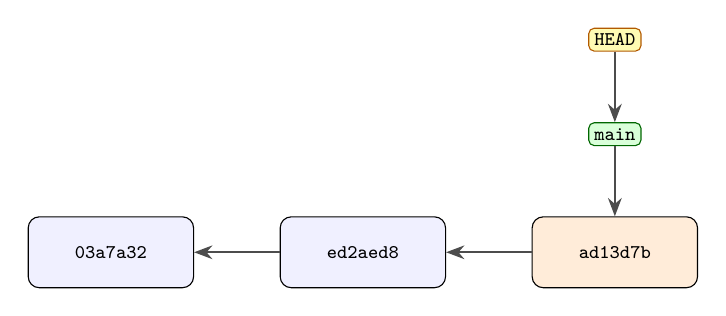
\begin{tikzpicture}[
  cbx/.style={draw,rounded corners,fill=blue!6,minimum width=2.1cm,minimum height=9mm,align=center,font=\scriptsize\ttfamily,inner sep=2pt}]
  \node[cbx] (a) at (0,0)   {03a7a32};
  \node[cbx] (b) at (3.2,0) {ed2aed8};
  \node[cbx,fill=orange!15] (c) at (6.4,0) {ad13d7b};
  \draw[link] (b)--(a); \draw[link] (c)--(b);
  \node[branchtag] (m) at (6.4,1.5) {main};
  \node[headtag]   (h) at (6.4,2.7) {HEAD};
  \draw[link] (m)--(c);
  \draw[link] (h)--(m);
\end{tikzpicture}
\caption{Three commits. The branch \code{main} points at the newest one. \code{HEAD} points at the branch you are on.}
\label{fig:pointer}
\end{figure}

\begin{lstlisting}
$ git log --oneline --decorate
ad13d7b (HEAD -> main) Add crepe recipe
ed2aed8 Add pancake recipe
03a7a32 Add README
\end{lstlisting}

The words in brackets are the labels attached to a commit: \code{HEAD -> main} means ``\code{HEAD} points at \code{main}, which points here''. (Your terminal shows these automatically; if it does not, add \code{--decorate}.)

In Lecture 3 we said \code{HEAD} is ``the commit you are on''. Now the full story: \textbf{\code{HEAD} points at the \emph{current branch}, and the branch points at a commit.} When you make a commit, Git creates the new commit and moves the \emph{current branch} label forward to it. Nothing else moves.

\begin{quickfact}
Because a branch is only a 40-character commit ID in a tiny file, creating one takes a few milliseconds and almost no space, however large the project is. In some older systems a branch meant copying the whole project, which is why branching was slow and rare. In Git it is so cheap that you should use branches freely.
\end{quickfact}

\section{Creating and switching}

\begin{lstlisting}
$ git branch
* main
$ git branch waffles
$ git branch
* main
  waffles
\end{lstlisting}

\code{git branch} lists the branches; the star marks the one you are on. \code{git branch waffles} creates a new branch \emph{at the commit you are on} but does not move you. Both labels now point at the same commit:

\begin{lstlisting}
$ git log --oneline --decorate
ad13d7b (HEAD -> main, waffles) Add crepe recipe
ed2aed8 Add pancake recipe
03a7a32 Add README
\end{lstlisting}

To move onto the new branch, \code{switch} to it:

\begin{lstlisting}
$ git switch waffles
Switched to branch 'waffles'
\end{lstlisting}

\begin{figure}[H]
\centering
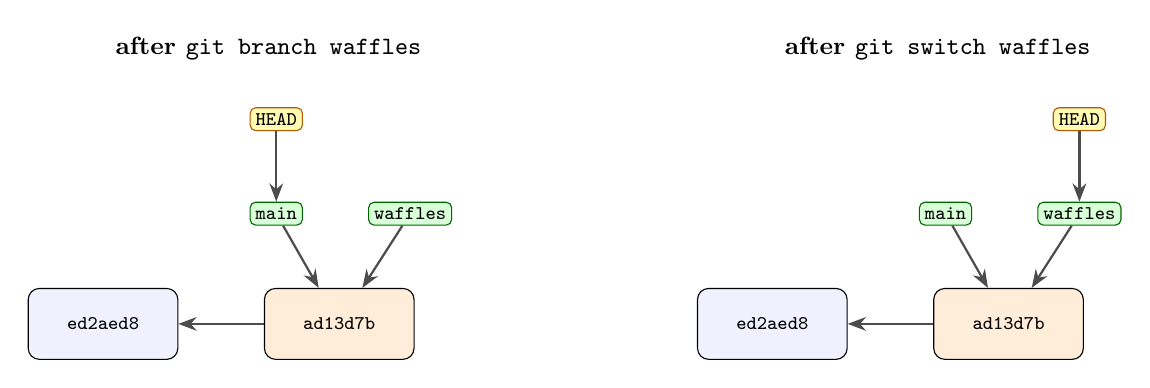
\begin{tikzpicture}[
  cbx/.style={draw,rounded corners,fill=blue!6,minimum width=1.9cm,minimum height=9mm,align=center,font=\scriptsize\ttfamily,inner sep=2pt}]
  % panel a
  \node[font=\small\bfseries] at (2.1,3.5) {after \code{git branch waffles}};
  \node[cbx] (b1) at (0,0)   {ed2aed8};
  \node[cbx,fill=orange!15] (c1) at (3.0,0) {ad13d7b};
  \draw[link] (c1)--(b1);
  \node[branchtag] (m1) at (2.2,1.4) {main};
  \node[branchtag] (w1) at (3.9,1.4) {waffles};
  \node[headtag]   (h1) at (2.2,2.6) {HEAD};
  \draw[link] (m1)--(c1); \draw[link] (w1)--(c1); \draw[link] (h1)--(m1);
  % panel b
  \node[font=\small\bfseries] at (10.6,3.5) {after \code{git switch waffles}};
  \node[cbx] (b2) at (8.5,0)   {ed2aed8};
  \node[cbx,fill=orange!15] (c2) at (11.5,0) {ad13d7b};
  \draw[link] (c2)--(b2);
  \node[branchtag] (m2) at (10.7,1.4) {main};
  \node[branchtag] (w2) at (12.4,1.4) {waffles};
  \node[headtag]   (h2) at (12.4,2.6) {HEAD};
  \draw[link] (m2)--(c2); \draw[link] (w2)--(c2); \draw[link] (h2)--(w2);
\end{tikzpicture}
\caption{Creating a branch adds a second label to the same commit. Switching moves only \code{HEAD}. No files are copied.}
\label{fig:create}
\end{figure}

The two steps are so common that there is a shortcut: \code{git switch -c waffles} \textbf{c}reates the branch and switches to it in one go. To see which branch you are on, \code{git status} says \code{On branch ...} on its first line, and \code{git branch --show-current} prints just the name.

\begin{quickfact}
\code{git switch} arrived in Git 2.23 (2019). Before that, one command did several jobs: \code{git checkout waffles} switched branches and \code{git checkout -b waffles} created one. You will meet \code{checkout} in many tutorials; for switching branches it does the same as \code{switch}. We use \code{switch} because it does one thing only.
\end{quickfact}

\subsection{Choosing a name}

Branch names should be short, lowercase and descriptive of the idea, with hyphens instead of spaces: \code{waffles}, \code{fix-typo}, \code{add-login}. Spaces are not allowed, and a slash is fine for grouping (\code{feature/login}). Use one branch per idea.

\section{Committing on a branch}

We are on \code{waffles}. Add a recipe and commit:

\begin{lstlisting}
$ echo "Waffles: flour, milk, eggs, sugar" >> recipes.txt
$ git add recipes.txt
$ git commit -m "Add waffle recipe"
$ git log --oneline --decorate
12c4aa1 (HEAD -> waffles) Add waffle recipe
ad13d7b (main) Add crepe recipe
ed2aed8 Add pancake recipe
03a7a32 Add README
\end{lstlisting}

(The new ID will be different on your computer, because it depends on the time of the commit.) Git created the commit and moved the \emph{current} branch, \code{waffles}, forward. \code{main} did not move:

\begin{figure}[H]
\centering
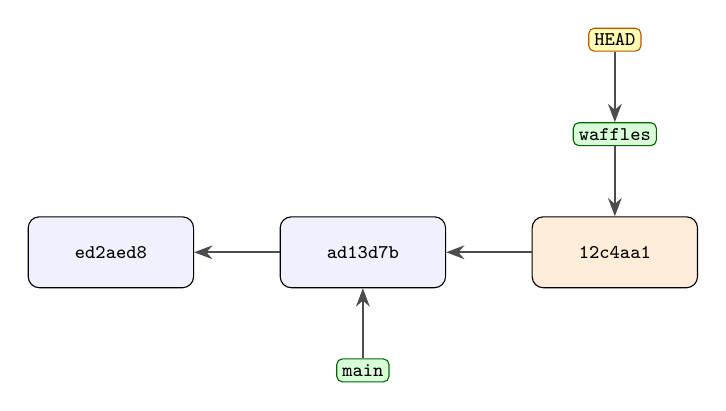
\begin{tikzpicture}[
  cbx/.style={draw,rounded corners,fill=blue!6,minimum width=2.1cm,minimum height=9mm,align=center,font=\scriptsize\ttfamily,inner sep=2pt}]
  \node[cbx] (a) at (0,0)   {ed2aed8};
  \node[cbx] (b) at (3.2,0) {ad13d7b};
  \node[cbx,fill=orange!15] (c) at (6.4,0) {12c4aa1};
  \draw[link] (b)--(a); \draw[link] (c)--(b);
  \node[branchtag] (m) at (3.2,-1.5) {main};
  \node[branchtag] (w) at (6.4,1.5) {waffles};
  \node[headtag]   (h) at (6.4,2.7) {HEAD};
  \draw[link] (m)--(b); \draw[link] (w)--(c); \draw[link] (h)--(w);
\end{tikzpicture}
\caption{After one commit on \code{waffles}. Only the current branch label moved.}
\label{fig:commit}
\end{figure}

\subsection{Switching changes your files}

Your working directory always shows the files of the commit that the current branch points at. When you switch, Git rewrites your files to match:

\Needspace{8\baselineskip}
\begin{lstlisting}
$ cat recipes.txt          # on waffles
Pancakes: flour, milk, eggs
Crepes: flour, milk, eggs, butter
Waffles: flour, milk, eggs, sugar
$ git switch main
Switched to branch 'main'
$ cat recipes.txt          # the waffle line is gone
Pancakes: flour, milk, eggs
Crepes: flour, milk, eggs, butter
\end{lstlisting}

The waffle recipe is not lost: it is saved in the commit that \code{waffles} points to. Switch back and the file returns. This is the superpower of branches: one folder, several versions of the project, one command to change between them.

\begin{tryit}
In \code{demo4}, switch between \code{main} and \code{waffles} a few times, each time running \code{cat recipes.txt} and \code{git status}. Watch the file change, and note that \code{git status} always names the current branch.
\end{tryit}

\section{Diverging history}

Now work on \code{main} as well. We are on \code{main} after the switch; add a muffin recipe:

\begin{lstlisting}
$ echo "Muffins: flour, milk" >> recipes.txt
$ git add recipes.txt
$ git commit -m "Add muffin recipe"
$ git log --oneline --decorate --all --graph
* d3cf462 (HEAD -> main) Add muffin recipe
| * 12c4aa1 (waffles) Add waffle recipe
|/
* ad13d7b Add crepe recipe
* ed2aed8 Add pancake recipe
* 03a7a32 Add README
\end{lstlisting}

The history has \emph{forked}. Both new commits have the crepe commit as their parent, but neither knows about the other.

\begin{figure}[H]
\centering
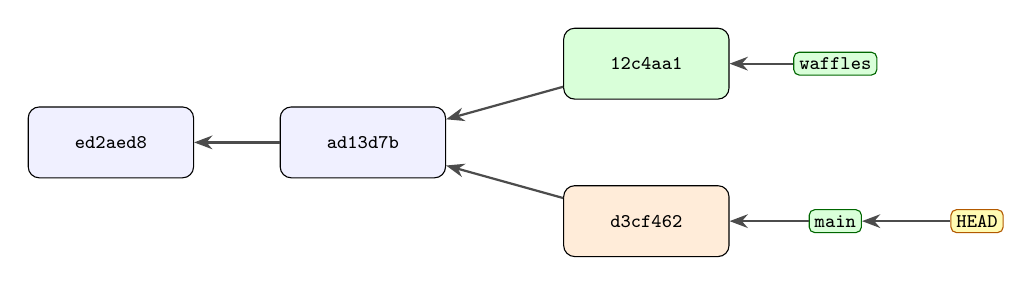
\begin{tikzpicture}[
  cbx/.style={draw,rounded corners,fill=blue!6,minimum width=2.1cm,minimum height=9mm,align=center,font=\scriptsize\ttfamily,inner sep=2pt}]
  \node[cbx] (a) at (0,0)   {ed2aed8};
  \node[cbx] (b) at (3.2,0) {ad13d7b};
  \node[cbx,fill=green!15]  (w) at (6.8,1.0)  {12c4aa1};
  \node[cbx,fill=orange!15] (m) at (6.8,-1.0) {d3cf462};
  \draw[link] (b)--(a); \draw[link] (w)--(b); \draw[link] (m)--(b);
  \node[branchtag] (wt) at (9.2,1.0)  {waffles};
  \node[branchtag] (mt) at (9.2,-1.0) {main};
  \node[headtag]   (ht) at (11.0,-1.0) {HEAD};
  \draw[link] (wt)--(w); \draw[link] (mt)--(m); \draw[link] (ht)--(mt);
\end{tikzpicture}
\caption{Two branches that have diverged. Each has a commit the other lacks. Lecture 5 combines them.}
\label{fig:diverge}
\end{figure}

To read the graph: each \code{*} is a commit; the lines show how commits connect; the labels in brackets are branch names. \code{--all} shows every branch (without it, \code{git log} shows only the history of the current one) and \code{--graph} draws the lines. This is the command to run whenever you wonder ``what does my history look like?''

\begin{lstlisting}
$ git branch -v
* main    d3cf462 Add muffin recipe
  waffles 12c4aa1 Add waffle recipe
\end{lstlisting}

\code{git branch -v} lists each branch with the commit it points to.

\begin{pitfall}
The most common branch mistake is committing on the wrong branch because you forgot which one you were on. Before you commit, check the first line of \code{git status}. (If it happens, Lecture 8 shows how to move the commit.)
\end{pitfall}

\section{Switching with uncommitted changes}

What happens if you have edited files and switch? Git protects your work. Two cases:

\textbf{The branches do not disagree about the files you changed.} The changes simply come along:

\begin{lstlisting}
$ echo "draft" > ideas.txt          # a brand-new file
$ git switch waffles
Switched to branch 'waffles'
$ git status --short
?? ideas.txt
\end{lstlisting}

(Switch back with \code{git switch main} and delete the file with \code{rm ideas.txt} before the next example.)

\textbf{The target branch has a different version of a file you edited.} Git refuses rather than overwrite your edit:

\begin{lstlisting}
$ echo "Scones: flour, butter" >> recipes.txt
$ git switch waffles
error: Your local changes to the following files would be overwritten by checkout:
	recipes.txt
Please commit your changes or stash them before you switch branches.
Aborting
\end{lstlisting}

Nothing has changed: you are still on \code{main}, and your edit is intact. (To continue with the lecture, discard the experiment with \code{git restore recipes.txt}.) In a real situation you have three options: \emph{commit} the change (the usual choice), \emph{discard} it with \code{git restore recipes.txt} if it was junk (Lecture 3), or save it for later with \code{git stash} (Lecture 10).

\begin{keyidea}
Good habit: commit, or at least check \code{git status}, before you switch branches. A clean working directory makes switching always safe.
\end{keyidea}

\section{More branch commands}

\begin{center}
\small
\begin{tabular}{@{}l >{\raggedright\arraybackslash}p{9.4cm}@{}}
\toprule
Command & What it does \\
\midrule
\code{git switch -c name start} & Create a branch that starts at \code{start}, a commit ID or another branch (for example \code{ed2aed8} or \code{main\textasciitilde{}1}), and switch to it. Without \code{start} it begins at the current commit. \\
\code{git branch name start} & The same, but do not switch. \\
\code{git branch -m old new} & Rename a branch (\textbf{m}ove). \\
\code{git branch -d name} & Delete a branch, but only if its work is safely included in another branch. \\
\bottomrule
\end{tabular}
\end{center}

\Needspace{9\baselineskip}
\begin{lstlisting}
$ git branch experiment ed2aed8
$ git branch -m experiment trial
$ git branch -d trial
Deleted branch trial (was ed2aed8).
$ git branch -d waffles
error: The branch 'waffles' is not fully merged.
If you are sure you want to delete it, run 'git branch -D waffles'.
\end{lstlisting}

The first deletion worked because \code{trial} points at a commit that is already part of \code{main}, so nothing would be lost. \code{waffles} has a commit that exists nowhere else, so Git refuses.

\begin{pitfall}
Deleting a branch deletes only the label, never the files in your folder. But the commits that only that branch pointed to become unreachable. That is why \code{-d} refuses to delete a branch with work that exists nowhere else, as above. \code{git branch -D} forces the deletion. Do not use \code{-D} until you understand why (Lecture 10 shows how such commits can still be rescued for a while). For now, if Git refuses, believe it. (The exact wording of the error varies a little between Git versions.)
\end{pitfall}

The usual life cycle is: create, work, merge (Lecture 5), delete with \code{-d}.

\section{Detached HEAD: looking at an old commit}

Sometimes you want to look at an old commit. \code{git switch --detach} puts \code{HEAD} on a commit directly, not on a branch:

\begin{lstlisting}
$ git switch --detach HEAD~1
HEAD is now at ad13d7b Add crepe recipe
$ git log --oneline --decorate -2
ad13d7b (HEAD) Add crepe recipe
ed2aed8 Add pancake recipe
\end{lstlisting}

\begin{figure}[H]
\centering
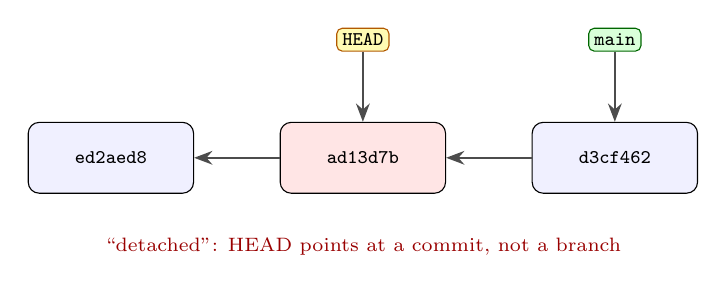
\begin{tikzpicture}[
  cbx/.style={draw,rounded corners,fill=blue!6,minimum width=2.1cm,minimum height=9mm,align=center,font=\scriptsize\ttfamily,inner sep=2pt}]
  \node[cbx] (a) at (0,0)   {ed2aed8};
  \node[cbx,fill=red!10] (b) at (3.2,0) {ad13d7b};
  \node[cbx] (c) at (6.4,0) {d3cf462};
  \draw[link] (b)--(a); \draw[link] (c)--(b);
  \node[branchtag] (m) at (6.4,1.5) {main};
  \draw[link] (m)--(c);
  \node[headtag] (h) at (3.2,1.5) {HEAD};
  \draw[link] (h)--(b);
  \node[font=\scriptsize,text=red!60!black,anchor=north] at (3.2,-0.9) {``detached'': HEAD points at a commit, not a branch};
\end{tikzpicture}
\caption{Detached HEAD. Looking around is fine, but a commit made now belongs to no branch.}
\label{fig:detached}
\end{figure}

Git calls this a \emph{detached HEAD}. It sounds alarming but is harmless as long as you only look. The danger: if you commit while detached, the new commit has no branch label, and when you switch away it becomes hard to find. To leave, just switch back: \code{git switch main}. If you \emph{did} make useful commits while detached, give them a branch straight away: \code{git switch -c rescue}.

\section{Homework 4}

\begin{homework}{4: Branching out}
From the course folder run:
\begin{lstlisting}
$ bash codeHints/L04/setup_hw4.sh
$ cd practice/hw4
\end{lstlisting}
You get two commits on \code{main} and a misspelled branch. Look with \code{git log --oneline --graph --all --decorate}. Do the tasks in order; to start over, run \code{setup\_hw4.sh --reset} from the course folder.

\begin{description}[leftmargin=1.2em,style=nextline]
\item[4.1 Branch] Create a branch \code{shopping} and switch to it.
\item[4.2 Work on it] On \code{shopping}, create \code{shopping.txt} containing \code{milk}; commit it as \code{Add shopping list}. Add a second line \code{eggs} and commit that as \code{Add eggs}.
\item[4.3 Back to main] Switch to \code{main}; check that \code{shopping.txt} is gone. Create \code{notes.txt} (any content) and commit it as \code{Add notes}.
\item[4.4 Rename] Fix the misspelled branch: rename \code{experimnt} to \code{experiment}. It must keep pointing at the first commit.
\item[4.5 Start point] Without switching, create a branch \code{hotfix} that points at the commit just before the newest commit on \code{main} (that is, at \code{main\textasciitilde{}1}).
\item[4.6 Finish and answer] Switch back to \code{main} and leave the working directory clean. In \code{practice/hw4\_answers.txt} (outside the repository) write two lines:
\begin{lstlisting}
branches=<how many branches the repository has now>
branch-is=<one word: what a branch is, technically>
\end{lstlisting}
\end{description}

Final graph: \code{main} and \code{shopping} fork at \code{Add app file}, where \code{hotfix} sits; \code{experiment} is on the first commit. \textbf{Check yourself:} from the course folder run \code{bash codeHints/L04/check\_hw4.sh}. All \code{PASS}, then compare with the solutions at the end of this lecture (or in \code{solutions/L04/}).
\end{homework}

\section{Summary}

\begin{itemize}
  \item A branch is a movable label pointing at a commit; \code{HEAD} points at the current branch. Committing moves the current branch forward.
  \item \code{git branch} lists, \code{git branch name} creates, \code{git switch name} moves, \code{git switch -c name} does both; \code{-m} renames, \code{-d} deletes safely.
  \item Switching rewrites your files to match the branch. Commit first; Git refuses to overwrite uncommitted edits.
  \item \code{git log --oneline --decorate --all --graph} shows all branches and where they diverge.
  \item A detached \code{HEAD} (on a commit, not a branch) is for looking only. Further reading: \emph{Pro Git}, Chapter 3.1.
\end{itemize}


\solutionspage

\section*{Solutions to Homework 4}

\begin{lstlisting}
$ bash codeHints/L04/setup_hw4.sh
$ cd practice/hw4
$ git switch -c shopping
$ echo "milk" > shopping.txt
$ git add shopping.txt
$ git commit -m "Add shopping list"
$ echo "eggs" >> shopping.txt
$ git add shopping.txt
$ git commit -m "Add eggs"
$ git switch main
$ ls                          # no shopping.txt here
README.md  app.txt
$ echo "some notes" > notes.txt
$ git add notes.txt
$ git commit -m "Add notes"
$ git branch -m experimnt experiment
$ git branch hotfix main~1
$ git log --oneline --graph --all --decorate
* c6fac68 (HEAD -> main) Add notes
| * e7fa817 (shopping) Add eggs
| * 26c01df Add shopping list
|/
* 2e32674 (hotfix) Add app file
* 0a964a7 (experiment) Initial commit
$ printf 'branches=4\nbranch-is=pointer\n' > ../hw4_answers.txt
\end{lstlisting}

(The first two IDs, \code{0a964a7} and \code{2e32674}, are the same on your computer; the others depend on when you commit and will differ.)

\textbf{4.1.} \code{git switch -c shopping} creates and enters the branch at the \code{Add app file} commit, where \code{main} is at that moment. Creating it \emph{before} the \code{Add notes} commit matters: the fork point is where the two lines of work separate.

\textbf{4.2.} Both commits go onto \code{shopping} because that is the branch \code{HEAD} points at. Check with \code{git status} (first line) before each commit.

\textbf{4.3.} After \code{git switch main} your files change: \code{shopping.txt} disappears from the folder. It is not lost; it lives in the commits of \code{shopping}. The \code{Add notes} commit moves \code{main} only. \code{shopping} stays where it was.

\textbf{4.4.} \code{git branch -m old new} renames. The branch still points at the first commit, so the checker's ``experiment is the first commit'' test passes.

\textbf{4.5.} \code{git branch hotfix main~1} creates the label at the parent of the newest \code{main} commit, which is \code{Add app file}, without switching. (\code{git switch -c} would also have created it, but you would then have to switch back.)

\textbf{4.6.} The four branches are \code{experiment}, \code{hotfix}, \code{main} and \code{shopping}. The word is \textbf{pointer}; ``label'' and ``reference'' are also accepted.

\Needspace{8\baselineskip}
\textbf{Common mistakes.}
\begin{itemize}
  \item Making the \code{shopping} commits while still on \code{main} (forgetting to switch). The checker then finds main with too many commits. Use \code{setup\_hw4.sh --reset} and start again, watching the first line of \code{git status}.
  \item Creating \code{shopping} \emph{after} the \code{Add notes} commit, so it forks from the wrong place.
  \item Using \code{git branch -D} or deleting \code{experimnt} instead of renaming it: the commit is still there but the branch name must be \code{experiment}.
  \item Ending the exercise on another branch: the last task asks you to be on \code{main}.
\end{itemize}


\end{document}
